\documentclass[10pt]{article}
\usepackage[a4paper,margin=0.84in]{geometry}
\usepackage[T1]{fontenc}
\usepackage{lmodern}
\usepackage{amsmath,amssymb,amsthm}
\usepackage{graphicx}
\usepackage{microtype}
\usepackage[colorlinks=true,linkcolor=blue,urlcolor=blue,citecolor=blue]{hyperref}
\newtheorem{theorem}{Theorem}
\newtheorem{lemma}{Lemma}
\newcommand{\Ric}{\operatorname{Ric}}
\newcommand{\vol}{\operatorname{vol}}
\newcommand{\C}{\mathbb C}

\title{A Berger-Five-Sphere Counterexample to Sharp\\
Spectral and Contraction Comparison}
\author{Candidate full counterexample packet\\
\small arXiv:1508.00606v4, Conjectures 3 and 4}
\date{11 August 2026}

\begin{document}
\maketitle

\paragraph{Status.}
Candidate full counterexample to both Conjectures~3 and~4 of Milman
\cite{Milman}, subject to expert review.  The final spectral certificate is
exact and occurs on a standard homogeneous Berger metric on $S^5$.

\section{Source questions}
Let $g_{\rm can}^{\rho}$ be the round metric on $S^n$ rescaled so that
$\Ric_{g_{\rm can}^{\rho}}=\rho g_{\rm can}^{\rho}$.  Milman's Conjecture~3
asks whether every metric $g$ on $S^n$ satisfying $\Ric_g\geq\rho g$ obeys
\begin{equation}\label{eq:source-spectral}
 \lambda_j(S^n,g)\geq\lambda_j(S^n,g_{\rm can}^{\rho})
 \qquad(j\geq1),
\end{equation}
where the source indexes the spectrum with $\lambda_1=0$.
Conjecture~4 asks more strongly for a metric contraction
\[
 T:(S^n,g_{\rm can}^{\rho},\vol_{g_{\rm can}^{\rho}})
 \longrightarrow(S^n,g,\vol_g)
\]
that pushes the first volume measure to a finite constant times the second
\cite[pp.~8--9]{Milman}.  Such a map implies \eqref{eq:source-spectral} by the
source's Contraction Principle.

\begin{figure}[ht]
\centering
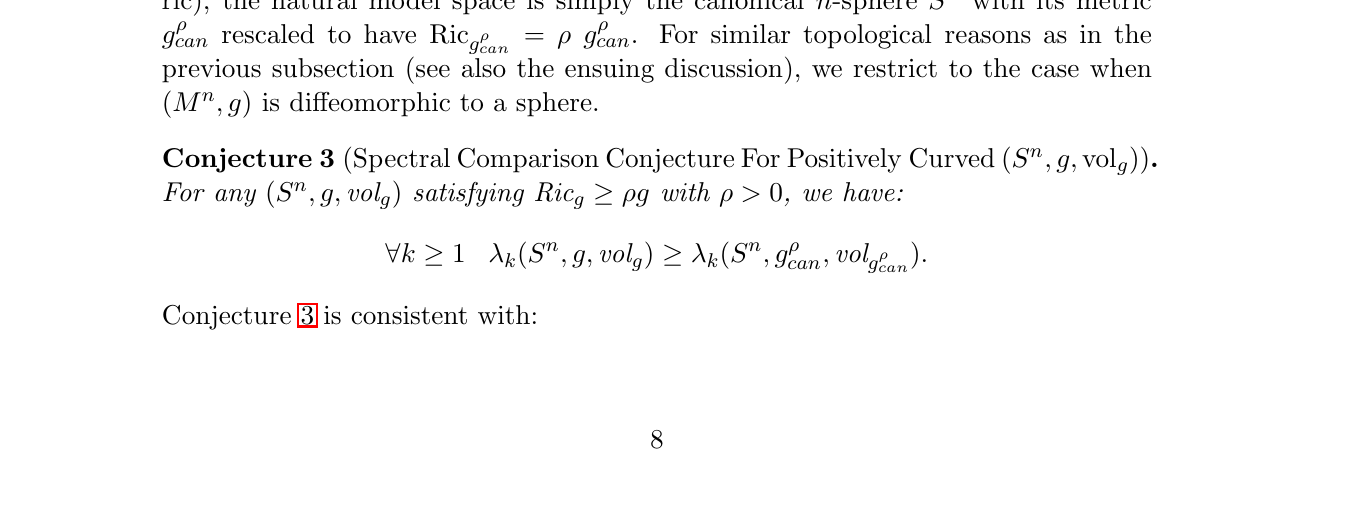
\includegraphics[width=.93\textwidth]{figures/conjecture3_crop.png}
\caption{Conjecture~3 in the source PDF, page~8.}
\end{figure}

\begin{figure}[ht]
\centering
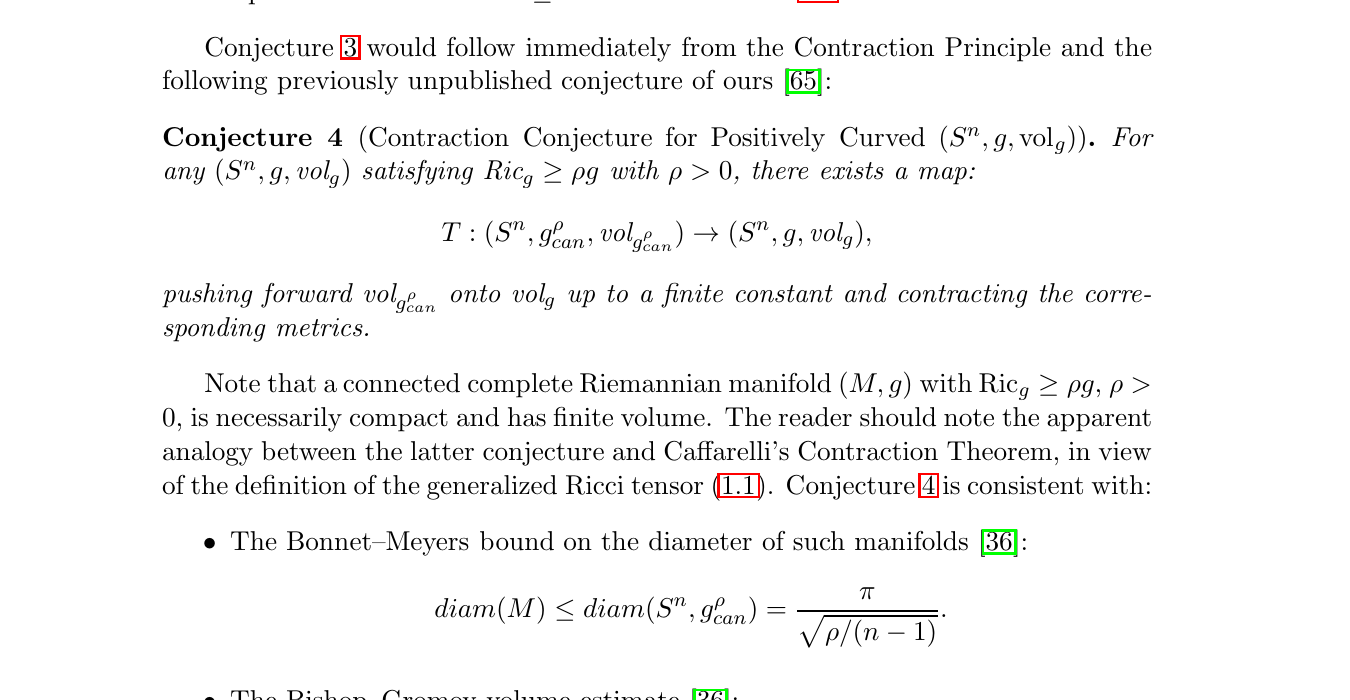
\includegraphics[width=.93\textwidth]{figures/conjecture4_crop.png}
\caption{The implication from Conjecture~4 to Conjecture~3 and the statement
of Conjecture~4, source PDF page~9.}
\end{figure}

\section{The Berger metric and proof intuition}
View the unit round sphere $S^5\subset\C^3$ as the total space of the complex
Hopf fibration $S^1\to S^5\to\C P^2$.  Its tangent bundle splits orthogonally
as $TS^5=\mathcal H\oplus\mathcal V$, where $\mathcal V$ is generated by the
unit Hopf field $\xi(z)=iz$.  If $g_0$ is the unit round metric, put
\begin{equation}\label{eq:berger}
 g_a=g_0|_{\mathcal H}+a\,g_0|_{\mathcal V},\qquad a=\frac54.
\end{equation}
Thus Hopf-fiber lengths are multiplied by $\sqrt a$.

\paragraph{Proof intuition.}
Stretching the Hopf fibers has two competing effects.  It decreases the
eigenvalues of functions with high circle weight, but it also decreases the
horizontal Ricci curvature and hence enlarges the round comparison sphere.
At low degrees the comparison rescaling wins.  At degree seven, however, the
purely holomorphic modes have enough Hopf weight to move below the corresponding
round level.  The degree-six and degree-seven clusters remain separated, so a
finite multiplicity count turns this crossing into an exact violation of the
ordered spectrum at index $715$.

\section{Geometric and spectral formulas}
We record the two standard canonical-variation calculations in the precise
normalization used here.  They may also be obtained from the Gray--O'Neill
formulas and the classical Berger-sphere spectral decomposition
\cite{Besse,Tanno}.

\begin{lemma}[Ricci tensor]\label{lem:ricci}
For $S^{2m+1}$ with $g_a=g_{\mathcal H}+a g_{\mathcal V}$, the Ricci
eigenvalues relative to $g_a$ are
\[
 r_{\mathcal H}=2m+2-2a,\qquad r_{\mathcal V}=2ma.
\]
For \eqref{eq:berger}, they are respectively $7/2$ and $5$.
\end{lemma}

\begin{proof}
For a $g_a$-unit horizontal vector $X$ and a $g_a$-unit vertical vector $U$,
the canonical-variation sectional curvatures are
\[
 K_a(X,U)=a,\qquad K_a(X,JX)=4-3a,
\]
and $K_a(X,Y)=1$ for horizontal $Y\perp\{X,JX\}$.  Summing over an
orthonormal frame gives
\[
 \Ric_a(X,X)=(4-3a)+(2m-2)+a=2m+2-2a,
 \quad \Ric_a(U,U)=2ma.
\]
Putting $m=2$ and $a=5/4$ gives $7/2$ and $5$.
\end{proof}

\begin{lemma}[Function spectrum]\label{lem:spectrum}
Let $\mathcal H_{p,q}$ be the restrictions to $S^{2m+1}$ of harmonic
polynomials on $\C^{m+1}$ that are homogeneous of degree $p$ in $z$ and degree
$q$ in $\bar z$.  On $\mathcal H_{p,q}$, the positive Laplacian of $g_a$ has
eigenvalue
\begin{equation}\label{eq:berger-eigen}
 \Lambda_a(p,q)=k(k+2m)+(a^{-1}-1)(p-q)^2,\qquad k=p+q.
\end{equation}
The direct sum over $p+q=k$ is the full round degree-$k$ spherical-harmonic
space.
\end{lemma}

\begin{proof}
The positive round Laplacian has eigenvalue $k(k+2m)$ on degree-$k$
spherical harmonics.  The Hopf generator satisfies
$\xi f=i(p-q)f$ on $\mathcal H_{p,q}$.  Scaling the vertical squared length by
$a$ changes the positive function Laplacian by
$(a^{-1}-1)(-\xi^2)$, which gives \eqref{eq:berger-eigen}.  The usual complex
bihomogeneous decomposition of harmonic polynomials gives the last assertion.
\end{proof}

\section{Exact counterexample}
\begin{theorem}\label{thm:main}
The Berger metric $g_{5/4}$ on $S^5$ satisfies
$\Ric_{g_{5/4}}\geq(7/2)g_{5/4}$, but
\[
 \lambda_{715}(S^5,g_{5/4})=\frac{336}{5}
 <\frac{539}{8}
 =\lambda_{715}(S^5,g_{\rm can}^{7/2}).
\]
The deficit is $7/40$.  Consequently Conjectures~3 and~4 of \cite{Milman}
are both false.
\end{theorem}

\begin{proof}
The Ricci assertion is Lemma~\ref{lem:ricci}.  Since the unit round $S^5$ has
$\Ric=4g_0$, its $(7/2)$-Ricci comparison metric is $(8/7)g_0$.  Its positive
Laplacian therefore has degree-$k$ eigenvalue
\begin{equation}\label{eq:round-eigen}
 \Lambda_{\rm cmp}(k)=\frac78 k(k+4).
\end{equation}

For $a=5/4$, Lemma~\ref{lem:spectrum} becomes
\begin{equation}\label{eq:target-eigen}
 \Lambda_{5/4}(p,q)=k(k+4)-\frac15(p-q)^2.
\end{equation}
The largest eigenvalue among all modes of degrees $0\leq k\leq6$ is at most
$6(6+4)=60$.  For fixed degree $k$, the smallest value in
\eqref{eq:target-eigen} occurs at $|p-q|=k$ and equals
\[
 F(k)=k(k+4)-\frac15k^2=\frac45k^2+4k.
\]
This is strictly increasing for $k\geq0$, and $F(7)=336/5>60$.  Hence every
mode of degree at most six precedes every mode of degree at least seven in the
ordered $g_{5/4}$ spectrum, and the first degree-seven value is $336/5$.  It
is attained, for instance, on nonzero holomorphic homogeneous polynomials of
degree seven, which are harmonic.

The dimension of the degree-$k$ spherical-harmonic space on $S^5$ is
\[
 d_k=\binom{k+5}{5}-\binom{k+3}{5},
\]
with the second term interpreted as zero for $k<2$.  For $k=0,\ldots,6$ this
gives
\[
 (d_0,\ldots,d_6)=(1,6,20,50,105,196,336),\qquad
 \sum_{k=0}^6d_k=714.
\]
Remembering that the source convention starts with $\lambda_1=0$, we obtain
\[
 \lambda_{715}(S^5,g_{5/4})=F(7)=\frac{336}{5}.
\]
The comparison sphere has the same degree multiplicities and strictly
increasing levels \eqref{eq:round-eigen}, so its 715th eigenvalue is its first
degree-seven value:
\[
 \lambda_{715}(S^5,g_{\rm can}^{7/2})
 =\frac78\,7(7+4)=\frac{539}{8}.
\]
Finally,
\[
 \frac{539}{8}-\frac{336}{5}=\frac7{40}>0,
\]
which disproves Conjecture~3.

For completeness, suppose a map from the comparison sphere to
$(S^5,g_{5/4})$ as in Conjecture~4 existed.  Pullback by this map is injective
on $L^2$ because its pushforward is a positive constant times target volume.
The metric contraction and the almost-everywhere chain rule give
\[
 \int |\nabla(f\circ T)|^2\,d\vol_{g_{\rm can}^{7/2}}
 \leq c\int|\nabla f|^2\,d\vol_{g_{5/4}},\qquad
 \int |f\circ T|^2\,d\vol_{g_{\rm can}^{7/2}}
 =c\int|f|^2\,d\vol_{g_{5/4}}
\]
for the same $c>0$.  The min--max principle would imply every comparison
eigenvalue is at most the corresponding target eigenvalue, contradicting the
715th-eigenvalue calculation.  Thus Conjecture~4 is false as well.
\end{proof}

\section{Verification, scope, and novelty}
The script \texttt{code/verify\_spectrum.py} uses exact rational arithmetic.
It checks the two Ricci values, the $7/8$ comparison scale, the
bihomogeneous multiplicities, the 714-mode count, degree separation, both
715th eigenvalues, and the exact $7/40$ deficit.  Its final output is:
\begin{verbatim}
Ricci eigenvalues (horizontal, vertical) = 7/2 5
modes of degrees 0 through 6 = 714
lambda_715(Berger S^5) = 336/5
lambda_715(round comparison S^5) = 539/8
strict deficit = 7/40
all exact checks passed
\end{verbatim}

The construction refutes the universal conjectures but does not classify the
dimensions or metric families where comparison survives.  In particular, Lin,
Wang, and Xu recently proved Conjecture~3 for all positively curved
two-spheres \cite{LWX}, and Serres proved a near-round two-sphere case of the
contraction statement \cite{Serres}; this example is five-dimensional and does
not conflict with either result.  It also does not contradict the source's heat
trace comparison or its asymptotic Weyl comparison: coordinatewise spectral
ordering is strictly stronger.

A bounded novelty search through 11 August 2026 covered the four run indexes;
the exact source id, title, and conjecture phrases; combinations of Milman's
name with ``Berger sphere'', ``spectral comparison'', and ``counterexample'';
citation-oriented searches; the 2018 journal page; and the two recent
two-sphere papers just cited.  It found no prior counterexample or this
calculation.  This is not a claim of priority.

\paragraph{Human-review recommendation.}
Very high priority.  Verify Lemmas~\ref{lem:ricci} and~\ref{lem:spectrum} in
the stated fiber-scaling convention.  Once those standard formulas are fixed,
the remaining proof is a short exact multiplicity count.

\begin{thebibliography}{9}
\bibitem{Milman}
E. Milman, \emph{Spectral estimates, contractions and hypercontractivity},
J. Spectr. Theory 8 (2018), 669--714;
\href{https://arxiv.org/abs/1508.00606}{arXiv:1508.00606v4}.

\bibitem{Besse}
A. L. Besse, \emph{Einstein Manifolds}, Springer, 1987, discussion of
canonical variations and Berger spheres.

\bibitem{Tanno}
S. Tanno, \emph{The first eigenvalue of the Laplacian on spheres},
Tohoku Math. J. 31 (1979), 179--185.

\bibitem{LWX}
S. Lin, H. Wang, and G. Xu, \emph{Eigenvalues on spheres},
\href{https://arxiv.org/abs/2607.11544}{arXiv:2607.11544} (2026).

\bibitem{Serres}
J. Serres, \emph{Contractive transport maps from $S^2$ to nearly spherical
surfaces with positive Ricci curvature},
\href{https://arxiv.org/abs/2508.13688}{arXiv:2508.13688} (2025).
\end{thebibliography}
\end{document}
